%!TEX root = ../../main.tex

\chapter{Long tasks}
Long running tasks should generally not block the GUI. Any task that can potentially take a long time should be done on a background thread and NOT on the main GUI thread see Appendix \ref{app:threading_asynctask}. 

Long running tasks should generally be supported by visual feedback which tells the user that something is going on and that the application is not frozen. 

\section{Progressbar}
The Android framework includes a widget called ProgressBar which can be used both as an activity indicator, see \ref{fig:activity_indicator_in_dialog}, and as an actual progress bar. ProgressBar is henceforth be reffered to as just ProgressBar, covering both usages, unless otherwise made explicit. Both are great at indicating that the app is not frozen and that something is going on. The ProgressBar (as a progress bar) should generally be used when there is a reliable way of calculating the actually progress og the running task. And the Activity indicator should generally be used when there is no way of telling how long there will be til the task is complete. 

\begin{figure}[!htbp]
  \centering
    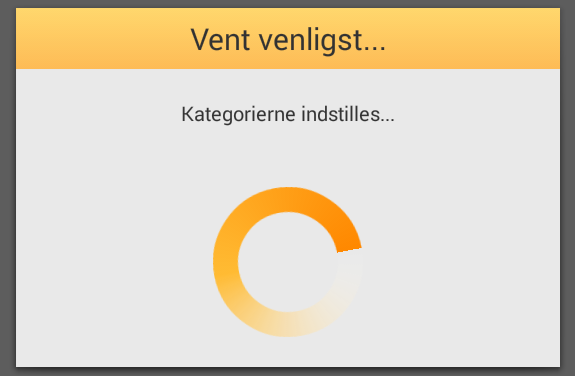
\includegraphics[width=0.8\textwidth]{progressbar_example}
    \caption{Example of a progress bar used as an activity indicator.}
    \label{fig:activity_indicator_in_dialog}
\end{figure}

If one have temporally unused screen real estate at the location where one are conceptually loading in elements then you should place you progress bar or activity indicator in this unused screen real estate.

\section{Dialogs}
One should use a Giraf dialog with a ProgressBar while the task is running if one does not have enough screen real estate available for a ProgressBar or if it otherwise does not make sense to place the ProgressBar in the layout.  